\documentclass[]{elsarticle} %review=doublespace preprint=single 5p=2 column
%%% Begin My package additions %%%%%%%%%%%%%%%%%%%
\usepackage[hyphens]{url}

  \journal{An awesome journal} % Sets Journal name


\usepackage{lineno} % add
\providecommand{\tightlist}{%
  \setlength{\itemsep}{0pt}\setlength{\parskip}{0pt}}

\bibliographystyle{elsarticle-harv}
\biboptions{sort&compress} % For natbib
\usepackage{graphicx}
\usepackage{booktabs} % book-quality tables
%%%%%%%%%%%%%%%% end my additions to header

\usepackage[T1]{fontenc}
\usepackage{lmodern}
\usepackage{amssymb,amsmath}
\usepackage{ifxetex,ifluatex}
\usepackage{fixltx2e} % provides \textsubscript
% use upquote if available, for straight quotes in verbatim environments
\IfFileExists{upquote.sty}{\usepackage{upquote}}{}
\ifnum 0\ifxetex 1\fi\ifluatex 1\fi=0 % if pdftex
  \usepackage[utf8]{inputenc}
\else % if luatex or xelatex
  \usepackage{fontspec}
  \ifxetex
    \usepackage{xltxtra,xunicode}
  \fi
  \defaultfontfeatures{Mapping=tex-text,Scale=MatchLowercase}
  \newcommand{\euro}{€}
\fi
% use microtype if available
\IfFileExists{microtype.sty}{\usepackage{microtype}}{}
\ifxetex
  \usepackage[setpagesize=false, % page size defined by xetex
              unicode=false, % unicode breaks when used with xetex
              xetex]{hyperref}
\else
  \usepackage[unicode=true]{hyperref}
\fi
\hypersetup{breaklinks=true,
            bookmarks=true,
            pdfauthor={},
            pdftitle={Evaluation of property price fluctuaction according to geographical landmarks, an Dublin case study},
            colorlinks=false,
            urlcolor=blue,
            linkcolor=magenta,
            pdfborder={0 0 0}}
\urlstyle{same}  % don't use monospace font for urls

\setcounter{secnumdepth}{0}
% Pandoc toggle for numbering sections (defaults to be off)
\setcounter{secnumdepth}{0}
% Pandoc header
\usepackage{float}
\usepackage{booktabs}
\usepackage{array}



\begin{document}
\begin{frontmatter}

  \title{Evaluation of property price fluctuaction according to geographical
landmarks, an Dublin case study}
    \author[Dublin City University]{Damien Dupré\corref{c1}}
   \ead{damien.dupre@dcu.ie} 
   \cortext[c1]{Corresponding Author}
      \address[Dublin City University]{Business School, Glasnevin, Dublin 9, Ireland}
  
  \begin{abstract}
  This is the abstract.
  
  It consists of two paragraphs.
  \end{abstract}
  
 \end{frontmatter}

\section{Introdution}\label{introdution}

To acquire a property is one of the most important achievement that
individuals are seeking. It provides not only a housing security but
also the feeling of being a landowner. However the access to the status
of landowner is complicated because buying a property is the most
expensive spending of in a lifetime. For this reason understanding the
factors which are explaining how property prices evolve is a necessity.

Due to its geographic, economic and political situation, Ireland in
general and Dublin in particular saw important changes in property
prices in the last ten years. From a economic boom known as the ``celtic
tiger'' in the 2000's, Ireland were deeply impacted by the 2007 economic
crisis. With an expected GDP growth of 4\% for 2019, property prices are
back to their highest. Whereas this grow is moderated in Irish mainland,
its capital Dublin is at the center of a housing crisis. Because of
factors including Irish economic wealth, the presence of tec companies
european headquarters such as Facebook or Google and the historic
configuration of the city which low population density structure and
underdeveloped public transportation, property prices became
unaffordable to most of irish families.

In this paper we want to identify the spatio-temporal factors that
influcenced the evolution of Dublin property prices. More precisely we
want to highlight not only macroeconomical influences such as GDP but
also the presence of econimical landmarks such as tec companies
headquarters and public transportation system on property prices
evoluation.

\section{Method}\label{method}

Since the 1st January 2010, under the Property Services (Regulation)
Act, all individuals aquering a property in Ireland has to declare it to
Property Services Regulatory Authority (PSRA). It includes Date of Sale,
Price and Address of all residential properties purchased in Ireland as
declared to the Revenue Commissioners for stamp duty purposes
(https://propertypriceregister.ie). It must be noticed that data is
filed electronically by persons doing the conveyancing of the property
on behalf of the purchaser and errors may occur when the data is being
filed. In order to evaluate the spacial distribution of the property
sold, a geocoding from the filled addresses to GPS coordinated was
performed using the OpenStreetMap API.

\begin{table}[!h]

\caption{\label{tab:dublin-sample-size}Size of the PSRA database for properties sold in Dublin County per year since 2010 aftering filtering the orignal database.}
\centering
\fontsize{8}{10}\selectfont
\begin{tabular}{rr}
\toprule
year & n\\
\midrule
2010 & 4819\\
2011 & 3745\\
2012 & 4910\\
2013 & 5577\\
2014 & 832\\
2015 & 9657\\
2016 & 10731\\
2017 & 11991\\
2018 & 10395\\
\bottomrule
\end{tabular}
\end{table}

By focusing on the property sold in Dublin, 111155 entries were recorded
since 2010. After having filtered properties not corresponding to
houses, properties for which address was not possible to geocode,
artefacts in geocodes and abertant value in sales price. From the
self-reported database, 62657 properties sold in Dublin between
2010-01-01 and 2018-11-30 was geocoded (Table
\ref{tab:dublin-sample-size}).

\section{Results}\label{results}

\begin{figure}[H]

{\centering \includegraphics{property_price_paper_new_files/figure-latex/distrib-plot-1} 

}

\caption{Distribution of the PSRA database (filtered).}\label{fig:distrib-plot}
\end{figure}

The average properties price is 330364 euros (SD = 180448). In order to
remove potential human errors and outliers, prices higher or lower than
1 SD were removed from the original dataset (Figure
\ref{fig:distrib-plot}).

\begin{figure}[H]

{\centering 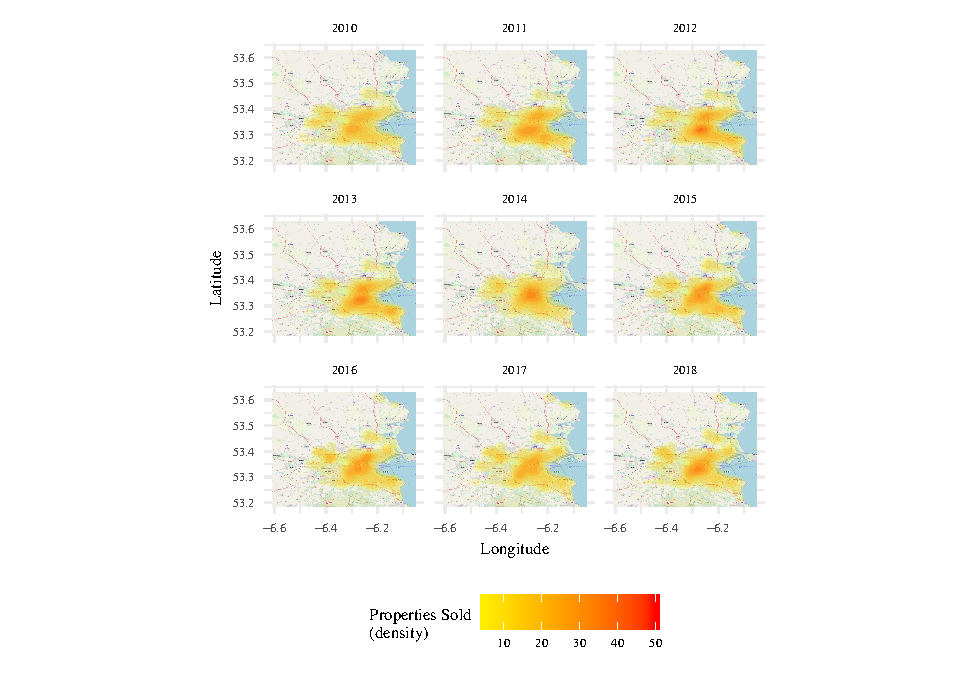
\includegraphics{property_price_paper_new_files/figure-latex/density-plot-1} 

}

\caption{Geographical density of the PSRA database (filtered).}\label{fig:density-plot}
\end{figure}

The distribution of properties sold in Dublin indicates that most of the
properties sold are located around Dublin 6 and Dublin 6 West districts
for every year investigated (Figure \ref{fig:density-plot}). However in
order to evaluate and to predict the distribution of housing prices, a
generalised additive model with model soap film smoothers (Wood,
Bravington and Hedley, 2008) is computed on the Dublin area. Soap film
smoothers are constructing a 2-D smooth prediction of non-linear
parameters such as latitude and longitude. The smooths are designed to
fit geographical models including coastal boundaries.

In order to model the distibution of properties, a Generalized Additive
Model using gaussian scale family for Soap film smooths was calculated
to fit the price of properties sold according to their GPS coordinates.
The result indicates that 20.3\% of property prices is explained by
property localisation (\emph{F}(62657,60.95) = 214.97; \emph{p}
\textless{} 0.001).

\begin{figure}[H]

{\centering \includegraphics{property_price_paper_new_files/figure-latex/gam-plot-1} 

}

\caption{Prediction of property price according the GAM model.}\label{fig:gam-plot}
\end{figure}

The Generalized Additive Model reveal not only high prices located on
the coast of Dublin (i.e Dublin 4 and Dun Laoghaire) but also a spot in
Dublin 7 which was un expected.

\subsection{Prediction of property price using
XGBoost}\label{prediction-of-property-price-using-xgboost}

In order to increase the prediction accuracy of the Generalized Additive
Model an XGBoost regression was performed on 195 geographic, economic
and social features.

\subsubsection{Geographical feature extraction using Open Street
Map}\label{geographical-feature-extraction-using-open-street-map}

Open Street map is a collaborative project which aims to create and
provide access to free editable maps of the world. Open Street Map
combines informations about more than 1177 features including road
informations and building informations to categorize amenities, leisure
or tourism structure for example. Among the 1177 features only 143
contain data for the Dublin Area (See list of Open Street Map features
in Appendix 1). In order to process the XGBoost regression the distance
between each property and the closest point corresponding to each of the
143 relevant Open Street Map.

\textbackslash{}begin\{table\}{[}!h{]}

\textbackslash{}caption\{\label{tab:OSM_features}Open Street Map
features importance (higher than 1\%).\} \centering
\fontsize{8}{10}\selectfont

\begin{tabular}{ll}
\toprule
Feature & Importance\\
\midrule
amenity\_embassy & 16.9\%\\
natural\_grassland & 6.3\%\\
route\_bus & 2.1\%\\
power\_line & 1.8\%\\
boundary\_administrative & 1.8\%\\
barrier\_wall & 1.7\%\\
cycleway\_lane & 1.7\%\\
amenity\_bar & 1.5\%\\
place\_island & 1.5\%\\
boundary\_political & 1.4\%\\
boundary\_historic & 1.4\%\\
cutting\_yes & 1.1\%\\
barrier\_full-height\_turnstile & 1.1\%\\
area\_yes & 1.1\%\\
route\_road & 1.1\%\\
place\_locality & 1.1\%\\
tunnel\_yes & 1.1\%\\
junction\_roundabout & 1.0\%\\
cycleway\_track & 1.0\%\\
barrier\_hedge & 1.0\%\\
route\_ferry & 1.0\%\\
\bottomrule
\end{tabular}

\textbackslash{}end\{table\}

\subsubsection{Economic and social feature extraction using Irish
census}\label{economic-and-social-feature-extraction-using-irish-census}

The results of Irish 2011 census consulation is accessible through the
All-Island Research Observatory (http://airo.maynoothuniversity.ie/) and
can be mapped over ireland small area boundaries which are fraction of
irish Electoral Division map. The social features extracted are
corresponding to population information, religion, carers and health.
Economic features correspond to the type of each small area including
the proportion of housing type, rooms number, occupancy and tenure per
small area. Each property is then associated to the value corresponding
to its small area.

\textbackslash{}begin\{table\}{[}!h{]}

\textbackslash{}caption\{\label{tab:AIRO_features}Census features
importance (higher than 1\%).\} \centering
\fontsize{8}{10}\selectfont

\begin{tabular}{ll}
\toprule
Feature & Importance\\
\midrule
\% 8 or more Rooms (Households) & 29.4\%\\
PC\_NO\_REL & 5.3\%\\
PCAGE014T & 4.2\%\\
\% Very Good & 3.4\%\\
\% 6 Rooms (Households) & 3.1\%\\
PCAGE80P & 2.9\%\\
\% 5 Rooms (Households) & 2.2\%\\
PC\_OTH\_C & 2.1\%\\
PC\_NS & 2.0\%\\
\% 3 Rooms (Households) & 2.0\%\\
\% Social Rented & 2.0\%\\
\% 7 Rooms (Households) & 1.9\%\\
\% Owner Occupier No Mortgage (Households) & 1.9\%\\
\% Persons with a disability aged 0-14 & 1.8\%\\
\% Private Rented & 1.8\%\\
\% Owner Occupier with Mortgage (Households) & 1.7\%\\
PC\_RO\_CATH & 1.7\%\\
\% Good & 1.7\%\\
PCAGE4564 & 1.6\%\\
\% 4 Rooms (Households) & 1.6\%\\
\% Persons with a disability aged 25 - 44 & 1.6\%\\
\% Persons with a disability aged 65 Plus & 1.6\%\\
\% Bad & 1.6\%\\
\% 1 Room (Households) & 1.4\%\\
PCAGE1524T & 1.3\%\\
\% Provides No Care & 1.3\%\\
PCAGE2544T & 1.3\%\\
PC\_FEMALE & 1.2\%\\
\% Persons with a disability aged 45 - 64 & 1.2\%\\
\% Occupied/HS With ususal Residents & 1.2\%\\
PCAEG65P & 1.2\%\\
\% House/Bungalow & 1.1\%\\
\bottomrule
\end{tabular}

\textbackslash{}end\{table\}

\section{Conclusion}\label{conclusion}

Using Generalized Additive Model we were able to identify the influence
of property locations based in Dublin, Ireland on their actual sale
price.

\section{Appendix}\label{appendix}

\begin{table}[t]

\caption{\label{tab:all_OSM_features}Relevant Open Street Map features for dublin area.}
\centering
\fontsize{8}{10}\selectfont
\begin{tabular}{l>{\raggedright\arraybackslash}p{3in}}
\toprule
Feature Category & Feature Type\\
\midrule
amenity & bar, college, school, university, bicycle parking, fuel, parking, community centre, bench, embassy, police, prison, recycling\\
barrier & city wall, ditch, fence, guard rail, hedge, kerb, retaining wall, wall, block, bollard, chain, full-height turnstile, gate, jersey barrier, yes\\
boundary & administrative, historic, political, postal code, protected area\\
building & apartments, house, residential, commercial, industrial, retail, hospital, university, yes\\
highway & motorway, trunk, secondary, tertiary, unclassified, residential, service, motorway link, trunk link, secondary link, tertiary link, pedestrian, track, road, footway, steps, path, cycleway\\
cycleway & lane, opposite, opposite lane, track, share busway, shared lane\\
busway & lane\\
highway & proposed, construction\\
junction & roundabout\\
historic & yes\\
landuse & commercial, construction, industrial, residential, retail, farmland, grass, military, railway, recreation ground, religious\\
leisure & nature reserve, park, slipway, sports centre, stadium, track\\
man made & breakwater, crane, embankment, groyne, pier, pipeline\\
natural & wood, tree row, scrub, grassland, water, beach, coastline, ridge, cliff\\
place & district, county, city, suburb, island, locality\\
power & cable, line, minor line, portal\\
line & busbar\\
public transport & platform, stop area\\
railway & abandoned, disused, rail, tram, platform\\
bridge & yes\\
cutting & yes\\
electrified contact & line\\
embankment & yes\\
service & crossover, siding, spur, yard\\
tunnel & yes\\
usage & main\\
route & bicycle, bus, ferry, hiking, power, road, train, tram\\
shop & paint, kitchen,\\
sport & badminton, equestrian, gaelic games, rugby union, running\\
tourism & artwork, zoo\\
waterway & river, riverbank, stream, canal, drain, ditch, weir, lock gate\\
source & survey\\
area & yes\\
covered & yes\\
disused & yes\\
tidal & yes\\
\bottomrule
\end{tabular}
\end{table}

\section*{References}\label{references}
\addcontentsline{toc}{section}{References}

\end{document}


